\documentclass[11pt,a4paper]{article}

% ============================================================
% PACKAGES
% ============================================================
\usepackage[utf8]{inputenc}
\usepackage[T1]{fontenc}
\usepackage[english]{babel}
\usepackage{amsmath, amssymb, amsthm}
\usepackage{geometry}
\geometry{margin=2.5cm}
\usepackage{graphicx}
\usepackage{xcolor}
\usepackage{listings}
\usepackage{hyperref}
\usepackage{booktabs}
\usepackage{array}
\usepackage{tikz}
\usetikzlibrary{arrows.meta, positioning, shapes, calc}

% ============================================================
% CONFIGURATION
% ============================================================
\hypersetup{
    colorlinks=true,
    linkcolor=blue,
    urlcolor=blue,
    citecolor=blue
}

\lstset{
    language=Python,
    basicstyle=\ttfamily\small,
    keywordstyle=\color{blue}\bfseries,
    commentstyle=\color{gray}\itshape,
    stringstyle=\color{red!70!black},
    numbers=left,
    numberstyle=\tiny\color{gray},
    frame=single,
    breaklines=true,
    showstringspaces=false,
    tabsize=4,
    literate={≤}{{$\leq$}}1 {≥}{{$\geq$}}1 {≠}{{$\neq$}}1
}

\newtheorem{theorem}{Theorem}[section]
\newtheorem{definition}[theorem]{Definition}
\newtheorem{lemma}[theorem]{Lemma}
\newtheorem{corollary}[theorem]{Corollary}
\newtheorem{example}[theorem]{Example}
\newtheorem{proposition}[theorem]{Proposition}

\newcommand{\bigO}{\mathcal{O}}
\newcommand{\bigOmega}{\Omega}
\newcommand{\bigTheta}{\Theta}
\newcommand{\code}[1]{\texttt{\detokenize{#1}}}

% ============================================================
% TITLE
% ============================================================
\title{\textbf{Algorithms: Complexity and Optimization}\\
\large Course Notes}
\author{}
\date{}

\begin{document}

\maketitle

\tableofcontents
\newpage

% ============================================================
% 1. INTRODUCTION
% ============================================================
\section{Introduction}

\subsection{Why Study Algorithms?}

An \textbf{algorithm} is a finite sequence of well-defined instructions that solves a computational problem. The same problem can often be solved by many different algorithms, and choosing the right one is the difference between a program that finishes in milliseconds and one that runs for years.

\begin{example}
Suppose you need to find a specific book in a library. If the books are organized randomly, you might have to check every single book --- that is, examine all $n$ books. If the books are sorted alphabetically, you can go directly to the right shelf and check only a few titles. The \emph{organization} of the data determines how fast you can find what you need.
\end{example}

This simple idea --- that the structure of the data determines the efficiency of the operations --- is the foundation of algorithm analysis.

\subsection{The Two Central Questions}

This course addresses two fundamental questions:

\begin{enumerate}
    \item \textbf{How do we measure the efficiency of an algorithm?}\\
    Answer: through \emph{asymptotic complexity analysis} (time and space).
    
    \item \textbf{How do we choose the right data structure and algorithm for a given problem?}\\
    Answer: by understanding the \emph{trade-offs} between structures and the \emph{paradigms} behind algorithms.
\end{enumerate}

\subsection{The Course Philosophy}

Throughout this course, we follow one principle:

\begin{quote}
\textbf{The mathematics decides, the code implements.}
\end{quote}

An algorithm is not optimized by tweaking code, but by changing its \emph{complexity class} --- and proving that no better class is possible.

% ============================================================
% 2. ASYMPTOTIC NOTATION
% ============================================================
\section{Asymptotic Notation and Complexity}

\subsection{Growth of Functions}

When analyzing algorithms, we care about how the running time grows as the input size $n$ increases. Constants and lower-order terms become negligible for large $n$.

\begin{center}
\begin{tabular}{c|cccccc}
\toprule
$n$ & $O(1)$ & $O(\log n)$ & $O(n)$ & $O(n \log n)$ & $O(n^2)$ & $O(2^n)$ \\
\midrule
10 & 1 & 3 & 10 & 33 & 100 & 1,024 \\
100 & 1 & 7 & 100 & 700 & 10,000 & $\sim 10^{30}$ \\
1,000 & 1 & 10 & 1,000 & 10,000 & 1,000,000 & astronomical \\
1,000,000 & 1 & 20 & $10^6$ & $2 \times 10^7$ & $10^{12}$ & impossible \\
\bottomrule
\end{tabular}
\end{center}

\subsection{Simple Examples of Each Complexity Class}

To build intuition, here are simple, well-known algorithms for each class.

\begin{example}[$O(1)$ --- constant time]
Accessing an element by index in an array:
\begin{lstlisting}
def get(arr, i):
    return arr[i]
\end{lstlisting}
The time does not depend on the size of the array. Whether the array has 10 or 10 million elements, accessing \code{arr[i]} takes the same number of operations (one multiplication, one addition, one memory read).
\end{example}

\begin{example}[$O(\log n)$ --- logarithmic time]
Dichotomy (binary search) in a sorted array: at each step, the search space is halved. We will analyze this in detail in Section~4.
\end{example}

\begin{example}[$O(n)$ --- linear time]
Finding the maximum of an array:
\begin{lstlisting}
def find_max(arr):
    m = arr[0]
    for x in arr:
        if x > m:
            m = x
    return m
\end{lstlisting}
We examine each element exactly once, so the time is proportional to $n$.
\end{example}

\begin{example}[$O(n \log n)$ --- linearithmic time]
Merge sort: we divide the array in half, sort each half, and merge. We will analyze this in Section~5.
\end{example}

\begin{example}[$O(n^2)$ --- quadratic time]
Checking whether all pairs of elements in an array sum to a target:
\begin{lstlisting}
def has_pair_sum(arr, target):
    for i in range(len(arr)):
        for j in range(i + 1, len(arr)):
            if arr[i] + arr[j] == target:
                return True
    return False
\end{lstlisting}
The outer loop runs $n$ times, the inner loop runs at most $n$ times, so there are at most $n^2$ comparisons.
\end{example}

\begin{example}[$O(2^n)$ --- exponential time]
Computing the $n$-th Fibonacci number by naive recursion:
\begin{lstlisting}
def fib_naive(n):
    if n <= 1:
        return n
    return fib_naive(n - 1) + fib_naive(n - 2)
\end{lstlisting}
Each call branches into two, so the number of calls doubles at each level. We will analyze this in detail in Section~2.4.
\end{example}

\subsection{Definitions}

\begin{definition}[Big-O --- upper bound]
$f(n) = \bigO(g(n))$ if there exist constants $c > 0$ and $n_0 > 0$ such that for all $n \geq n_0$:
\[
f(n) \leq c \cdot g(n).
\]
\end{definition}

\begin{definition}[Big-Omega --- lower bound]
$f(n) = \bigOmega(g(n))$ if there exist constants $c > 0$ and $n_0 > 0$ such that for all $n \geq n_0$:
\[
f(n) \geq c \cdot g(n).
\]
\end{definition}

\begin{definition}[Big-Theta --- tight bound]
$f(n) = \bigTheta(g(n))$ if $f(n) = \bigO(g(n))$ and $f(n) = \bigOmega(g(n))$.
\end{definition}

\begin{definition}[Little-o --- strict upper bound]
$f(n) = o(g(n))$ if for every constant $c > 0$, there exists $n_0 > 0$ such that for all $n \geq n_0$:
\[
f(n) < c \cdot g(n).
\]
Equivalently, $\lim_{n \to \infty} \frac{f(n)}{g(n)} = 0$.
\end{definition}

\begin{example}
Prove that $3n^2 + 5n + 7 = \bigO(n^2)$.

\textbf{Proof.} Choose $c = 15$ and $n_0 = 1$. For all $n \geq 1$:
\[
3n^2 + 5n + 7 \leq 3n^2 + 5n^2 + 7n^2 = 15n^2.
\]
Therefore $3n^2 + 5n + 7 = \bigO(n^2)$. \hfill $\blacksquare$
\end{example}

\begin{example}
$n = o(n^2)$ because $\lim_{n \to \infty} n/n^2 = 0$.
\end{example}


\begin{figure}[h]
\centering
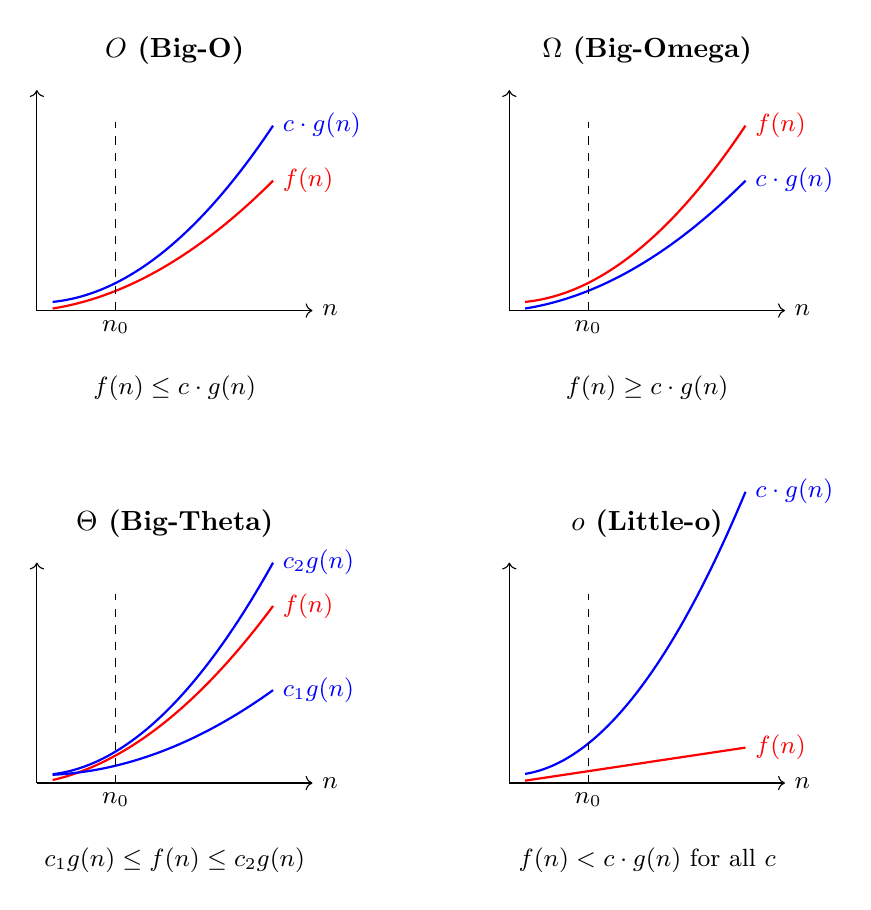
\begin{tikzpicture}[scale=1]

    % ========== FIRST LINE: O and Omega ==========

    % ---------- O (Big-O) ----------
    \begin{scope}[shift={(0,0)}]
        \draw[->] (0,0) -- (3.5,0) node[right] {\small $n$};
        \draw[->] (0,0) -- (0,2.8) node[above] {};
        % c*g(n) = c * n^2 — upper bound
        \draw[thick, blue, domain=0.2:3.0, samples=100] 
            plot (\x, {0.25*\x*\x + 0.1});
        \node[blue, right] at (3.0, {0.25*9 + 0.1}) {\small $c \cdot g(n)$};
        % f(n) = 0.15 n^2 + 0.3 n — smaller parabola
        \draw[thick, red, domain=0.2:3.0, samples=100] 
            plot (\x, {0.15*\x*\x + 0.1*\x});
        \node[red, right] at (3.0, {0.15*9 + 0.1*3}) {\small $f(n)$};
        % n0
        \draw[dashed] (1.0, 0) -- (1.0, 2.4);
        \node[below] at (1.0, 0) {\small $n_0$};
        % Title
        \node[above] at (1.75, 3.0) {\textbf{$O$ (Big-O)}};
        \node[below] at (1.75, -0.7) {\small $f(n) \leq c \cdot g(n)$};
    \end{scope}

    % ---------- Omega (Big-Omega) ----------
    \begin{scope}[shift={(6,0)}]
        \draw[->] (0,0) -- (3.5,0) node[right] {\small $n$};
        \draw[->] (0,0) -- (0,2.8) node[above] {};
        % f(n) = 0.25 n^2 + 0.1 — above
        \draw[thick, red, domain=0.2:3.0, samples=100] 
            plot (\x, {0.25*\x*\x + 0.1});
        \node[red, right] at (3.0, {0.25*9 + 0.1}) {\small $f(n)$};
        % c*g(n) = 0.15 n^2 + 0.1 n — lower bound
        \draw[thick, blue, domain=0.2:3.0, samples=100] 
            plot (\x, {0.15*\x*\x + 0.1*\x});
        \node[blue, right] at (3.0, {0.15*9 + 0.1*3}) {\small $c \cdot g(n)$};
        % n0
        \draw[dashed] (1.0, 0) -- (1.0, 2.4);
        \node[below] at (1.0, 0) {\small $n_0$};
        % Title
        \node[above] at (1.75, 3.0) {\textbf{$\Omega$ (Big-Omega)}};
        \node[below] at (1.75, -0.7) {\small $f(n) \geq c \cdot g(n)$};
    \end{scope}

    % ========== SECOND LINE: Theta and o ==========

    % ---------- Theta (Big-Theta) ----------
    \begin{scope}[shift={(0,-6.0)}]
        \draw[->] (0,0) -- (3.5,0) node[right] {\small $n$};
        \draw[->] (0,0) -- (0,2.8) node[above] {};
        % c2*g(n) = 0.30 n^2 + 0.1 — upper parabola
        \draw[thick, blue, domain=0.2:3.0, samples=100] 
            plot (\x, {0.30*\x*\x + 0.1});
        \node[blue, right] at (3.0, {0.30*9 + 0.1}) {\small $c_2 g(n)$};
        % f(n) = 0.20 n^2 + 0.2 n — middle
        \draw[thick, red, domain=0.2:3.0, samples=100] 
            plot (\x, {0.20*\x*\x + 0.15*\x});
        \node[red, right] at (3.0, {0.20*9 + 0.15*3}) {\small $f(n)$};
        % c1*g(n) = 0.12 n^2 + 0.1 — lower parabola
        \draw[thick, blue, domain=0.2:3.0, samples=100] 
            plot (\x, {0.12*\x*\x + 0.1});
        \node[blue, right] at (3.0, {0.12*9 + 0.1}) {\small $c_1 g(n)$};
        % n0
        \draw[dashed] (1.0, 0) -- (1.0, 2.4);
        \node[below] at (1.0, 0) {\small $n_0$};
        % Title
        \node[above] at (1.75, 3.0) {\textbf{$\Theta$ (Big-Theta)}};
        \node[below] at (1.75, -0.7) {\small $c_1 g(n) \leq f(n) \leq c_2 g(n)$};
    \end{scope}

    % ---------- o (Little-o) ----------
    \begin{scope}[shift={(6,-6.0)}]
        \draw[->] (0,0) -- (3.5,0) node[right] {\small $n$};
        \draw[->] (0,0) -- (0,2.8) node[above] {};
        % c*g(n) = 0.40 n^2 + 0.1 — big parabola
        \draw[thick, blue, domain=0.2:3.0, samples=100] 
            plot (\x, {0.40*\x*\x + 0.1});
        \node[blue, right] at (3.0, {0.40*9 + 0.1}) {\small $c \cdot g(n)$};
        % f(n) = 0.15 n — linear, much smaller
        \draw[thick, red, domain=0.2:3.0, samples=100] 
            plot (\x, {0.15*\x});
        \node[red, right] at (3.0, {0.15*3}) {\small $f(n)$};
        % n0
        \draw[dashed] (1.0, 0) -- (1.0, 2.4);
        \node[below] at (1.0, 0) {\small $n_0$};
        % Title
        \node[above] at (1.75, 3.0) {\textbf{$o$ (Little-o)}};
        \node[below] at (1.75, -0.7) {\small $f(n) < c \cdot g(n)$ for all $c$};
    \end{scope}

\end{tikzpicture}
\label{fig:notations}
\end{figure}




\subsection{Space Complexity}

The same notation applies to \textbf{space}: the amount of memory used by an algorithm as a function of $n$.

\begin{example}[Fibonacci numbers]
Consider three ways to compute the $n$-th Fibonacci number $F(n)$, where $F(0)=0$, $F(1)=1$, and $F(n) = F(n-1) + F(n-2)$.

\textbf{Naive recursion.}
\begin{lstlisting}
def fib_naive(n):
    if n <= 1:
        return n
    return fib_naive(n - 1) + fib_naive(n - 2)
\end{lstlisting}
Time complexity is $O(2^n)$ because each call branches into two. Space complexity is $O(n)$ --- the maximum depth of the recursion stack.

\textbf{Iterative with memoization (dynamic programming).}
\begin{lstlisting}
def fib_memo(n, memo={}):
    if n in memo:
        return memo[n]
    if n <= 1:
        return n
    memo[n] = fib_memo(n - 1, memo) + fib_memo(n - 2, memo)
    return memo[n]
\end{lstlisting}
Time complexity is $O(n)$. Space complexity is $O(n)$ for the memo dictionary and the recursion stack.

\textbf{Iterative with constant space.}
\begin{lstlisting}
def fib_iter(n):
    if n <= 1:
        return n
    a, b = 0, 1
    for _ in range(2, n + 1):
        a, b = b, a + b
    return b
\end{lstlisting}
Time complexity is $O(n)$. Space complexity is $O(1)$ --- only two variables are stored, regardless of $n$.
\end{example}

This example shows that the same problem can be solved with the same time complexity but different space complexities. The choice depends on the available memory.

\subsection{Common Pitfalls}

\begin{itemize}
    \item Constants do not matter: $\bigO(2n) = \bigO(n)$.
    \item Lower-order terms do not matter: $\bigO(n^2 + n) = \bigO(n^2)$.
    \item Best case $\neq$ lower bound: the best case is about a specific input; the lower bound is about all algorithms for a problem.
    \item $\bigO(n + m) \neq \bigO(n)$ if $m$ is independent.
\end{itemize}

% ============================================================
% 3. DATA STRUCTURES
% ============================================================
\section{Data Structures}

A \textbf{data structure} is a way of organizing data in memory to support efficient operations. The choice of data structure determines the complexity of every operation.

\subsection{Arrays}

An \textbf{array} is a contiguous block of memory storing elements of the same type.

\begin{center}
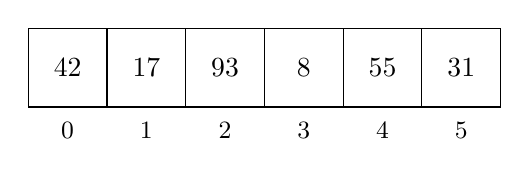
\begin{tikzpicture}
\foreach \i/\v in {0/42, 1/17, 2/93, 3/8, 4/55, 5/31} {
    \draw (\i,0) rectangle (\i+1,1);
    \node at (\i+0.5,0.5) {\v};
    \node at (\i+0.5,-0.3) {\small \i};
}
\end{tikzpicture}
\end{center}

\begin{center}
\begin{tabular}{lc}
\toprule
Operation & Complexity \\
\midrule
Access by index & $O(1)$ \\
Search (unsorted) & $O(n)$ \\
Search (sorted, dichotomy) & $O(\log n)$ \\
Insert/delete at end & $O(1)$ amortized \\
Insert/delete in middle & $O(n)$ \\
\bottomrule
\end{tabular}
\end{center}

\textbf{Advantages}: cache-friendly, $O(1)$ access.\\
\textbf{Disadvantages}: $O(n)$ insertion/deletion in the middle, fixed size (or resize cost).

\subsection{Linked Lists}

A \textbf{linked list} is a sequence of nodes, each containing a value and a pointer to the next node.

\begin{center}
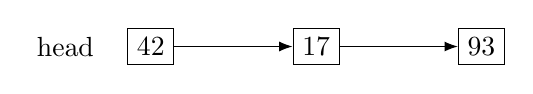
\begin{tikzpicture}[node distance=1.5cm]
\node[draw, rectangle] (n1) {42};
\node[draw, rectangle, right=of n1] (n2) {17};
\node[draw, rectangle, right=of n2] (n3) {93};
\draw[-{Latex}] (n1) -- (n2);
\draw[-{Latex}] (n2) -- (n3);
\node[left=0.3cm of n1] {head};
\end{tikzpicture}
\end{center}

\begin{center}
\begin{tabular}{lc}
\toprule
Operation & Complexity \\
\midrule
Access by index & $O(n)$ \\
Search & $O(n)$ \\
Insert/delete at head & $O(1)$ \\
Insert/delete after a node & $O(1)$ \\
\bottomrule
\end{tabular}
\end{center}

\textbf{Advantages}: $O(1)$ insertion/deletion, no resize cost.\\
\textbf{Disadvantages}: $O(n)$ access, poor cache locality.

\subsection{Stacks}

A \textbf{stack} is a LIFO (Last-In, First-Out) structure. Elements are added and removed from the same end, called the \emph{top}.

\begin{center}
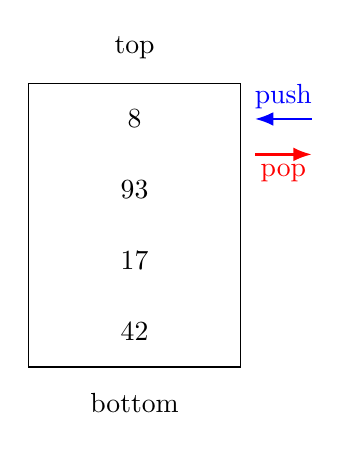
\begin{tikzpicture}[scale=0.9]
\draw (0,0) rectangle (3,4);
\node at (1.5,0.5) {42};
\node at (1.5,1.5) {17};
\node at (1.5,2.5) {93};
\node at (1.5,3.5) {8};
\draw[-{Latex}, thick, blue] (4,3.5) -- (3.2,3.5) node[midway, above] {push};
\draw[-{Latex}, thick, red] (3.2,3.0) -- (4,3.0) node[midway, below] {pop};
\node at (1.5,-0.5) {bottom};
\node at (1.5,4.5) {top};
\end{tikzpicture}
\end{center}

\begin{center}
\begin{tabular}{lc}
\toprule
Operation & Complexity \\
\midrule
Push & $O(1)$ \\
Pop & $O(1)$ \\
Peek & $O(1)$ \\
\bottomrule
\end{tabular}
\end{center}

\textbf{Implementation in Python}: \code{list} with \code{append} and \code{pop}. The \code{peek} operation reads the top element (\code{stack[-1]}) without removing it.

\subsection{Queues}

A \textbf{queue} is a FIFO (First-In, First-Out) structure. Elements are added at the \emph{rear} and removed from the \emph{front}.

\begin{center}
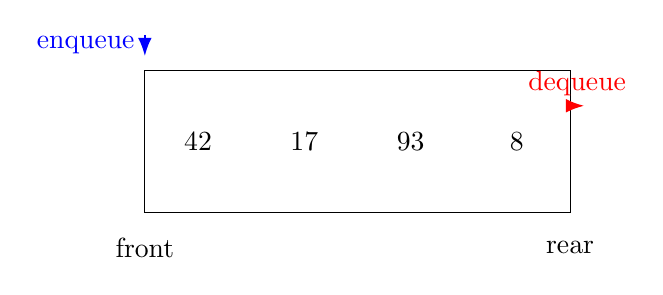
\begin{tikzpicture}[scale=0.9]
\draw (0,0) rectangle (6,2);
\node at (0.75,1) {42};
\node at (2.25,1) {17};
\node at (3.75,1) {93};
\node at (5.25,1) {8};
\draw[-{Latex}, thick, blue] (0,2.5) -- (0,2.2) node[midway, left] {enqueue};
\draw[-{Latex}, thick, red] (6,1.5) -- (6.2,1.5) node[midway, above] {dequeue};
\node at (0, -0.5) {front};
\node at (6, -0.5) {rear};
\end{tikzpicture}
\end{center}

\begin{center}
\begin{tabular}{lc}
\toprule
Operation & Complexity \\
\midrule
Enqueue & $O(1)$ \\
Dequeue & $O(1)$ \\
Peek & $O(1)$ \\
\bottomrule
\end{tabular}
\end{center}

\textbf{Implementation in Python}: \code{collections.deque} with \code{append} and \code{popleft}. The \code{peek} operation reads the front element (\code{queue[0]}) without removing it.

\subsection{Trees}

A \textbf{binary search tree} (BST) is a tree where, for every node, all keys in the left subtree are smaller, and all keys in the right subtree are larger.

\begin{center}
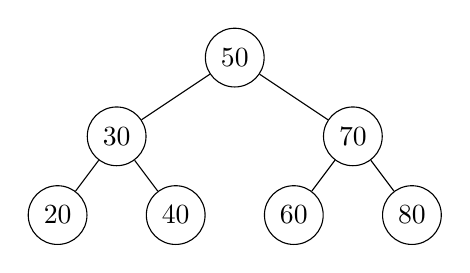
\begin{tikzpicture}[level distance=1cm, level 1/.style={sibling distance=3cm}, level 2/.style={sibling distance=1.5cm}]
\node[circle, draw] {50}
    child {node[circle, draw] {30}
        child {node[circle, draw] {20}}
        child {node[circle, draw] {40}}
    }
    child {node[circle, draw] {70}
        child {node[circle, draw] {60}}
        child {node[circle, draw] {80}}
    };
\end{tikzpicture}
\end{center}

\begin{center}
\begin{tabular}{lcc}
\toprule
Operation & Balanced BST & Degenerate BST \\
\midrule
Search & $O(\log n)$ & $O(n)$ \\
Insert & $O(\log n)$ & $O(n)$ \\
Delete & $O(\log n)$ & $O(n)$ \\
\bottomrule
\end{tabular}
\end{center}

\subsection{Graphs}

A \textbf{graph} $G = (V, E)$ is a set of vertices and edges.

\textbf{Representations}:
\begin{itemize}
    \item \textbf{Adjacency matrix}: $O(V^2)$ space, $O(1)$ edge test.
    \item \textbf{Adjacency list}: $O(V + E)$ space, $O(\deg(v))$ edge test.
\end{itemize}

\begin{center}
\begin{tabular}{lcc}
\toprule
Algorithm & List & Matrix \\
\midrule
BFS / DFS & $O(V + E)$ & $O(V^2)$ \\
\bottomrule
\end{tabular}
\end{center}

% ============================================================
% END OF PART 1
% ============================================================
% ============================================================
% 4. SEARCH IN BST AND SORTED LIST
% ============================================================
\section{Search in a BST and in a Sorted List}

\subsection{Dichotomy in a Sorted Array}

\textbf{Dichotomy} (binary search) is the principle of dividing the search space in half at each step. It requires the array to be sorted.

\subsubsection{Iterative version}

\begin{lstlisting}
def dichotomy_search(arr, x):
    lo, hi = 0, len(arr) - 1
    while lo <= hi:
        mid = (lo + hi) // 2
        if arr[mid] == x:
            return mid
        elif arr[mid] < x:
            lo = mid + 1
        else:
            hi = mid - 1
    return -1
\end{lstlisting}

\subsubsection{Recursive version}

\begin{lstlisting}
def dichotomy_search_recursive(arr, x, lo, hi):
    if lo > hi:
        return -1
    mid = (lo + hi) // 2
    if arr[mid] == x:
        return mid
    elif arr[mid] < x:
        return dichotomy_search_recursive(arr, x, mid + 1, hi)
    else:
        return dichotomy_search_recursive(arr, x, lo, mid - 1)
\end{lstlisting}

The recursive version has the same logic, but the recursive call is a \emph{tail call} --- it could be optimized into a loop by the compiler, but Python does not perform tail-call optimization. The iterative version is therefore preferred in practice.

\subsubsection{Complexity analysis in detail}

Let $T(n)$ be the number of comparisons performed by dichotomy on an array of size $n$. At each step, the algorithm performs \textbf{one comparison} (checking if \code{arr[mid] == x}) and then either stops or recurses on \textbf{half} of the remaining elements. Therefore:
\[
T(n) = T(n/2) + O(1).
\]

\textbf{Resolution by recurrence tree.}

At level 0, the problem has size $n$. At level 1, size $n/2$. At level 2, size $n/4$. In general, at level $k$, size $n/2^k$. The recursion stops when the size becomes 1 (or 0), i.e., when:
\[
\frac{n}{2^k} = 1 \quad \Longrightarrow \quad 2^k = n \quad \Longrightarrow \quad k = \log_2 n.
\]
So there are $\log_2 n$ levels. Each level performs $O(1)$ work (one comparison). Therefore:
\[
T(n) = O(1) \cdot \log_2 n = O(\log n).
\]

\textbf{Intuition: the halving argument.}

Each comparison eliminates \emph{half} of the remaining elements. Starting with $n$ elements, after 1 comparison at most $n/2$ remain, after 2 comparisons at most $n/4$, and after $k$ comparisons at most $n/2^k$. To reduce the search space to 1 element, we need:
\[
\frac{n}{2^k} \leq 1 \quad \Longrightarrow \quad k \geq \log_2 n.
\]
Therefore, at most $\lceil \log_2 n \rceil$ comparisons are needed. This is a \emph{worst-case} bound: the target might be at the last position examined, or absent entirely.

\begin{theorem}[Lower bound for comparison search]
Any comparison-based search in a sorted array of $n$ elements requires $\bigOmega(\log n)$ comparisons in the worst case.
\end{theorem}

\begin{proof}
The decision tree has $n$ leaves (one per element), so its depth $d$ satisfies $2^d \geq n$, hence $d \geq \log_2 n$.
\end{proof}

\textbf{Conclusion}: dichotomy is \emph{optimal} in the comparison model --- it achieves the lower bound $\bigOmega(\log n)$.

\subsection{Search in a BST}

\begin{lstlisting}
def bst_search(root, x):
    while root:
        if x == root.key:
            return root
        elif x < root.key:
            root = root.left
        else:
            root = root.right
    return None
\end{lstlisting}

\textbf{Complexity}: $O(h)$, where $h$ is the height of the tree.
\begin{itemize}
    \item Balanced BST: $h = O(\log n)$ $\Rightarrow$ search is $O(\log n)$.
    \item Degenerate BST: $h = O(n)$ $\Rightarrow$ search is $O(n)$.
\end{itemize}

\begin{definition}[AVL (Adelson-Velsky and Landis) Tree]
An \textbf{AVL tree} is a binary search tree in which, for every node $N$, the \emph{balance factor}
\[
\mathrm{balance}(N) = \mathrm{height}(N.\mathrm{left}) - \mathrm{height}(N.\mathrm{right})
\]
satisfies
\[
\mathrm{balance}(N) \in \{-1, 0, +1\}.
\]
\end{definition}

\begin{theorem}
An AVL tree with $n$ nodes has height $h \leq 1.44 \log_2 n + O(1)$.
\end{theorem}

\begin{proof}[Proof sketch]
Let $N(h)$ be the minimum number of nodes in an AVL tree of height $h$. To minimize nodes, the two subtrees have heights $h-1$ and $h-2$:
\[
N(h) = 1 + N(h-1) + N(h-2), \quad N(0) = 1, \quad N(1) = 2.
\]
The characteristic equation $x^2 = x + 1$ has root $\varphi = (1+\sqrt{5})/2$. Solving gives $N(h) \approx \varphi^{h+2}/\sqrt{5} - 1$. Inverting:
\[
h \leq \log_\varphi(\sqrt{5}(n+1)) - 2 = O(\log n).
\]
\end{proof}

% ============================================================
% 5. SORTING ALGORITHMS
% ============================================================
\section{Sorting Algorithms}

\subsection{Bubble Sort}

\begin{lstlisting}
def bubble_sort(arr):
    n = len(arr)
    for i in range(n):
        swapped = False
        for j in range(n - 1 - i):
            if arr[j] > arr[j + 1]:
                arr[j], arr[j + 1] = arr[j + 1], arr[j]
                swapped = True
        if not swapped:
            break
    return arr
\end{lstlisting}

\textbf{Complexity}:
\begin{itemize}
    \item Worst case: $O(n^2)$.
    \item Best case (sorted array): $O(n)$ (with the \code{swapped} flag).
    \item Space: $O(1)$.
\end{itemize}

\subsection{Quick Sort (Randomized Pivot)}

To avoid the worst case on sorted inputs, quick sort uses a \textbf{randomly chosen pivot}. The expected running time is $O(n \log n)$ regardless of the input distribution.

\subsubsection{List-based version (out of place)}

\begin{lstlisting}
import random

def quick_sort(arr):
    if len(arr) <= 1:
        return arr
    pivot_idx = random.randint(0, len(arr) - 1)
    pivot = arr[pivot_idx]
    left = [x for x in arr if x < pivot]
    mid = [x for x in arr if x == pivot]
    right = [x for x in arr if x > pivot]
    return quick_sort(left) + mid + quick_sort(right)
\end{lstlisting}

\textbf{Time complexity}:
\begin{itemize}
    \item Best/average case: $O(n \log n)$.
    \item Worst case: $O(n^2)$ (but with random pivot, this is extremely unlikely).
\end{itemize}

\textbf{Space complexity (this version)}: $O(n \log n)$ total allocations, $O(n)$ at any instant (the \code{left}, \code{mid}, \code{right} lists).

\subsubsection{In-place version with lo/hi tracking and pivot replacement}

The previous version allocates new lists at each recursive call. The \textbf{in-place} version uses two pointers, \code{i} and \code{j}, that move toward each other:

\begin{itemize}
    \item \code{i} tracks the \textbf{end of the low list} (elements $<$ pivot, on the left).
    \item \code{j} tracks the \textbf{start of the high list} (elements $>$ pivot, on the right).
\end{itemize}

The pivot is first placed at \code{arr[lo]}. The partition works by moving \code{i} right while elements are $<$ pivot, and \code{j} left while elements are $>$ pivot. When both stop, we swap \code{arr[i]} and \code{arr[j]}. When \code{i >= j}, the partition is complete, and we \textbf{place the pivot at its final position} \code{j} by swapping it with the element at that boundary.

\begin{lstlisting}
import random

def quick_sort_in_place(arr):
    _quick_sort(arr, 0, len(arr) - 1)
    return arr

def _quick_sort(arr, lo, hi):
    if lo >= hi:
        return
    p = _partition(arr, lo, hi)
    _quick_sort(arr, lo, p - 1)
    _quick_sort(arr, p + 1, hi)

def _partition(arr, lo, hi):
    # Random pivot: swap a random element with arr[lo]
    rand_idx = random.randint(lo, hi)
    arr[lo], arr[rand_idx] = arr[rand_idx], arr[lo]
    pivot = arr[lo]

    i = lo + 1   # end of the low list (elements < pivot)
    j = hi       # start of the high list (elements > pivot)

    while True:
        # Advance i while arr[i] < pivot
        while i <= j and arr[i] < pivot:
            i += 1
        # Retreat j while arr[j] > pivot
        while i <= j and arr[j] > pivot:
            j -= 1
        # If i >= j, the partition is complete
        if i >= j:
            break
        # Otherwise, swap arr[i] and arr[j]
        arr[i], arr[j] = arr[j], arr[i]
        i += 1
        j -= 1

    # Place the pivot at its final position: swap arr[lo] and arr[j]
    arr[lo], arr[j] = arr[j], arr[lo]
    return j
\end{lstlisting}

\textbf{How it works.} The pivot is placed at \code{arr[lo]}. The pointer \code{i} starts at \code{lo + 1} and advances while \code{arr[i] < pivot}. The pointer \code{j} starts at \code{hi} and retreats while \code{arr[j] > pivot}. When both stop, \code{arr[i]} is $\geq$ pivot and \code{arr[j]} is $\leq$ pivot --- they are on the wrong sides, so we swap them and advance both pointers. When \code{i >= j}, the partition is complete. At this point, \code{arr[lo]} (the pivot) is swapped with \code{arr[j]}, placing the pivot at its \textbf{final position} \code{j}. The recursive calls are then \code{_quick_sort(arr, lo, p - 1)} and \code{_quick_sort(arr, p + 1, hi)}, where \code{p = j}.

\textbf{Time complexity}:
\begin{itemize}
    \item Best/average case: $O(n \log n)$.
    \item Worst case: $O(n^2)$ (but with random pivot, this is extremely unlikely).
\end{itemize}

\textbf{Space complexity (in-place)}: $O(\log n)$ on average (recursion stack), $O(n)$ in the worst case. The array itself is modified in place --- no extra arrays are allocated.

\subsection{Merge Sort}

\begin{lstlisting}
def merge_sort(arr):
    if len(arr) <= 1:
        return arr
    mid = len(arr) // 2
    left = merge_sort(arr[:mid])
    right = merge_sort(arr[mid:])
    return merge(left, right)

def merge(left, right):
    result = []
    i = j = 0
    while i < len(left) and j < len(right):
        if left[i] <= right[j]:
            result.append(left[i])
            i += 1
        else:
            result.append(right[j])
            j += 1
    result.extend(left[i:])
    result.extend(right[j:])
    return result
\end{lstlisting}

\textbf{Recurrence}: $T(n) = 2T(n/2) + O(n)$, so $T(n) = O(n \log n)$.

\textbf{Complexity}:
\begin{itemize}
    \item All cases: $O(n \log n)$.
    \item Space: $O(n)$.
\end{itemize}

\subsection{Comparison Table}

\begin{center}
\begin{tabular}{lcccc}
\toprule
Algorithm & Best & Average & Worst & Space \\
\midrule
Bubble sort & $O(n)$ & $O(n^2)$ & $O(n^2)$ & $O(1)$ \\
Quick sort (random) & $O(n \log n)$ & $O(n \log n)$ & $O(n^2)$ & $O(n)$ \\
Quick sort (in place) & $O(n \log n)$ & $O(n \log n)$ & $O(n^2)$ & $O(\log n)$ \\
Merge sort & $O(n \log n)$ & $O(n \log n)$ & $O(n \log n)$ & $O(n)$ \\
\bottomrule
\end{tabular}
\end{center}

\subsection{Practical Timing Comparison on Large Data}

The following table shows the execution time of different complexity classes for large problem sizes, assuming one operation takes $1 \mu s$ (microsecond). This illustrates why the complexity class matters more than constant factors.

\begin{center}
\begin{tabular}{l|ccccc}
\toprule
Complexity & $n=1$ & $n=100$ & $n=10{,}000$ & $n=10^6$ & $n=10^9$ \\
\midrule
$\log_2 n$ & $1 \mu s$ & $7 \mu s$ & $13 \mu s$ & $20 \mu s$ & $30 \mu s$ \\
$n$ & $1 \mu s$ & $100 \mu s$ & $0.01 s$ & $1 s$ & $17$ minutes \\
$n \log_2 n$ & $1 \mu s$ & $700 \mu s$ & $0.13 s$ & $20 s$ & $8.5$ hours \\
$n^2$ & $1 \mu s$ & $0.01 s$ & $1.7$ minutes & $11.5$ days & $317$ centuries \\
$2^n$ & $1 \mu s$ & $10^{14}$ centuries & $\approx \infty$ & $\approx \infty$ & $\approx \infty$ \\
\bottomrule
\end{tabular}
\end{center}

\textbf{Interpretation}: for $n = 10^6$ (one million items), a linear algorithm ($O(n)$) finishes in 1 second, while a quadratic algorithm ($O(n^2)$) takes 11.5 days. An exponential algorithm ($O(2^n)$) would never finish. This is why choosing the right complexity class is not a theoretical exercise --- it has direct practical consequences.

% ============================================================
% 6. INSERTION AND DELETION
% ============================================================
\section{Insertion and Deletion}

\subsection{Insertion in an Array}

\begin{lstlisting}
def insert_at(arr, i, x):
    arr.append(None)
    for j in range(len(arr) - 1, i, -1):
        arr[j] = arr[j - 1]
    arr[i] = x
\end{lstlisting}

\textbf{Complexity}: $O(n)$ in the worst case (shifting elements).

\subsection{Insertion in a Linked List}

The nodes of a linked list are typically implemented as objects with two fields: the value they store, and a pointer to the next node. In Python, this is done with a simple class:

\begin{lstlisting}
class Node:
    def __init__(self, value):
        self.value = value
        self.next = None
\end{lstlisting}

The constructor \code{\_\_init\_\_} takes a value and stores it in the \code{value} attribute. The \code{next} attribute is initialized to \code{None}, meaning that the node does not yet point to any successor. When the node is inserted into a list, its \code{next} pointer is updated to reference the following node.

For example, the list \code{42 -> 17 -> 93} is built as follows:

\begin{lstlisting}
head = Node(42)
head.next = Node(17)
head.next.next = Node(93)
\end{lstlisting}

Each call to \code{Node(...)} creates a new node, and the \code{next} pointers are set to link the nodes together. The \code{head} variable holds a reference to the first node, which is the entry point to the entire list.

\begin{lstlisting}
def insert_after(node, x):
    new = Node(x)
    new.next = node.next
    node.next = new
\end{lstlisting}

\textbf{Complexity}: $O(1)$ (if the node is known).

\subsection{Insertion in a BST}

\begin{lstlisting}
def insert(root, key):
    if root is None:
        return Node(key)
    if key < root.key:
        root.left = insert(root.left, key)
    elif key > root.key:
        root.right = insert(root.right, key)
    return root
\end{lstlisting}

\textbf{Complexity}: $O(h)$, where $h$ is the height of the tree.

\subsection{Deletion in an Array}

\begin{lstlisting}
def delete_at(arr, i):
    for j in range(i, len(arr) - 1):
        arr[j] = arr[j + 1]
    arr.pop()
\end{lstlisting}

\textbf{Complexity}: $O(n)$.

\subsection{Deletion in a Linked List}

\begin{lstlisting}
def delete_after(node):
    if node.next:
        node.next = node.next.next
\end{lstlisting}

\textbf{Complexity}: $O(1)$.

\subsection{Deletion in a BST}

Three cases:
\begin{enumerate}
    \item \textbf{Leaf}: remove directly.
    \item \textbf{One child}: replace by the child.
    \item \textbf{Two children}: replace by the in-order successor.
\end{enumerate}

\begin{lstlisting}
def delete(root, key):
    if root is None:
        return root
    if key < root.key:
        root.left = delete(root.left, key)
    elif key > root.key:
        root.right = delete(root.right, key)
    else:
        if root.left is None:
            return root.right
        elif root.right is None:
            return root.left
        successor = find_min(root.right)
        root.key = successor.key
        root.right = delete(root.right, successor.key)
    return root
\end{lstlisting}

\textbf{Complexity}: $O(h)$.

% ============================================================
% 7. DIVIDE AND CONQUER: A UNIFYING VIEW
% ============================================================
\section{Divide and Conquer: A Unifying View}

The three algorithms studied in Section~4 (dichotomy) and Section~5 (merge sort and quick sort) share the same skeleton: \textbf{split} the problem, \textbf{solve} the parts recursively, \textbf{combine} the results. The differences lie in \emph{where the work happens}.

\begin{center}
\small
\begin{tabular}{lcccc}
\toprule
Algorithm & Split & Solve & Combine & Recurrence \\
\midrule
Dichotomy & Halve & Recurse on one half & None & $T(n) = T(n/2) + O(1)$ \\
Merge sort & Halve & Sort each half & Merge & $T(n) = 2T(n/2) + O(n)$ \\
Quick sort & Partition & Sort each side & None & $T(n) = T(k) + T(n{-}k{-}1) + O(n)$ \\
\bottomrule
\end{tabular}
\end{center}

\textbf{How to read the table.}
\begin{itemize}
    \item \textbf{Dichotomy}: the work is the comparison at each step; there is no combine step, because the search is already localized.
    \item \textbf{Merge sort}: the work is in the merge, which happens \emph{after} the recursive calls. This is the classical divide-and-conquer pattern: split first, solve, combine last.
    \item \textbf{Quick sort}: the work is in the partition, which happens \emph{before} the recursive calls. The recursive calls are on the two sides of the pivot, and there is no combine step, because the array is already in place.
\end{itemize}

\textbf{The recurrence column.} Each recurrence captures the cost of the algorithm as a function of the input size $n$:
\begin{itemize}
    \item $T(n) = T(n/2) + O(1)$: one recursive call on half the input, plus constant work.
    \item $T(n) = 2T(n/2) + O(n)$: two recursive calls on half the input, plus linear work.
    \item $T(n) = T(k) + T(n-k-1) + O(n)$: two recursive calls on sizes $k$ and $n-k-1$ (the pivot is excluded), plus linear work.
\end{itemize}

The first two recurrences resolve to $O(\log n)$ and $O(n \log n)$ respectively. The third resolves to $O(n \log n)$ in expectation when the pivot is chosen uniformly at random, and $O(n^2)$ in the worst case.

\textbf{Why this matters.} Divide and conquer is not a single algorithm --- it is a \emph{template}. The same template produces a search algorithm ($O(\log n)$), a sorting algorithm with guaranteed bounds (merge sort, $O(n \log n)$), and a sorting algorithm that is faster in practice but has a worse worst case (quick sort, $O(n^2)$ worst, $O(n \log n)$ expected). Recognizing the template is what allows us to design new algorithms for new problems.

% ============================================================
% 8. GREEDY ALGORITHMS
% ============================================================
\section{Greedy Algorithms}

\subsection{The Coin Change Problem (European System)}

\subsubsection{Statement}

Given a sum \( S \) and a set of coin denominations, find the \textbf{minimum number of coins} needed to make \( S \).

For the European system, the denominations are:
\[
\{1, 2, 5, 10, 20, 50\}.
\]

\begin{example}
\( S = 63 \). The optimal change is \( 50 + 10 + 2 + 1 \), which uses 4 coins.
\end{example}

\subsubsection{The Greedy Algorithm}

A \textbf{greedy algorithm} builds a solution \emph{step by step}, always making the choice that looks best \emph{at the moment}, without ever reconsidering past choices. The hope is that a sequence of locally optimal choices leads to a globally optimal solution.

Greedy algorithms are simple to design and often very fast, but they are \textbf{not always correct}. The central question of this section is: \emph{when is a greedy choice safe?}


The greedy strategy is: \emph{always take the largest coin that does not exceed the remaining sum}.

\begin{lstlisting}
def coin_change_greedy(S, coins=[50, 20, 10, 5, 2, 1]):
    used = {}
    for c in coins:
        count = S // c
        if count > 0:
            used[c] = count
        S %= c
    return used
\end{lstlisting}

The function returns a \textbf{dictionary} that maps each coin denomination to the number of times it is used. Coins that are not used do not appear in the dictionary.

\begin{example}
\( S = 63 \):
\begin{lstlisting}
>>> coin_change_greedy(63)
{50: 1, 10: 1, 2: 1, 1: 1}
\end{lstlisting}
This means: one coin of 50, one coin of 10, one coin of 2, and one coin of 1. The total number of coins is \( 1 + 1 + 1 + 1 = 4 \). The coins 20 and 5 are not used, so they do not appear in the dictionary.
\end{example}

\subsubsection{Complexity}

\textbf{Time:} \( O(k) \), where \( k \) is the number of denominations. Each denomination is processed once.

\textbf{Space:} \( O(k) \) for the dictionary (in the worst case, all denominations are used), plus \( O(1) \) for the counter and the remaining sum.

\subsubsection{Is the Greedy Choice Always Optimal?}

For the European system, \textbf{yes} --- it is a \emph{canonical} coin system, and the greedy algorithm produces the optimal change for every sum.

But this is \textbf{not true for all coin systems}. Consider the system \( \{1, 3, 4\} \) and \( S = 6 \):
\begin{itemize}
    \item Greedy: \( 4 + 1 + 1 \) = 3 coins.
    \item Optimal: \( 3 + 3 \) = 2 coins.
\end{itemize}
The greedy algorithm fails. This is the motivation for the dynamic programming approach in Section~9.

\subsection{Generating All Possible Changes (Tree Traversal)}

\subsubsection{Statement}

Instead of finding the \emph{minimum} number of coins, we now want to \textbf{enumerate all possible ways} to make a given sum \( S \) with a given set of coins. The order of the coins does \textbf{not} matter: two changes that use the same coins in a different order are considered the same.

\begin{example}
\( S = 4 \), coins \( \{1, 2\} \). The possible changes are:
\[
1+1+1+1, \quad 1+1+2, \quad 2+2.
\]
There are 3 ways (not 5, because the order does not matter).
\end{example}

\subsubsection{The Tree Traversal Algorithm}

To avoid generating the same change in different orders, we track the \textbf{last coin chosen} and only allow coins that are \textbf{less than or equal to} it. This enforces that the sequence of coins is non-increasing, so each combination is generated exactly once.

\begin{lstlisting}
def all_changes(S, coins):
    result = []

    def backtrack(remaining, current, last_coin):
        if remaining == 0:
            result.append(current[:])
            return
        for c in coins:
            if c <= remaining and c <= last_coin:
                current.append(c)
                backtrack(remaining - c, current, c)   # next coin <= c
                current.pop()   # undo (backtrack)

    backtrack(S, [], float('inf'))   # first call: any coin is allowed
    return result
\end{lstlisting}

\textbf{How it works.} The parameter \code{last\_coin} is the value of the last coin chosen (or \(+\infty\) for the first call). The condition \code{c <= last\_coin} ensures that the sequence of coins is non-increasing: after choosing a coin of value \(c\), we can only choose coins of value \(\leq c\). This prevents generating the same combination in different orders.

\subsubsection{\texorpdfstring{Example: Tree for \( S = 4 \), coins \( \{1, 2\} \)}{Example: Tree for S = 4, coins 1, 2}}

\begin{center}
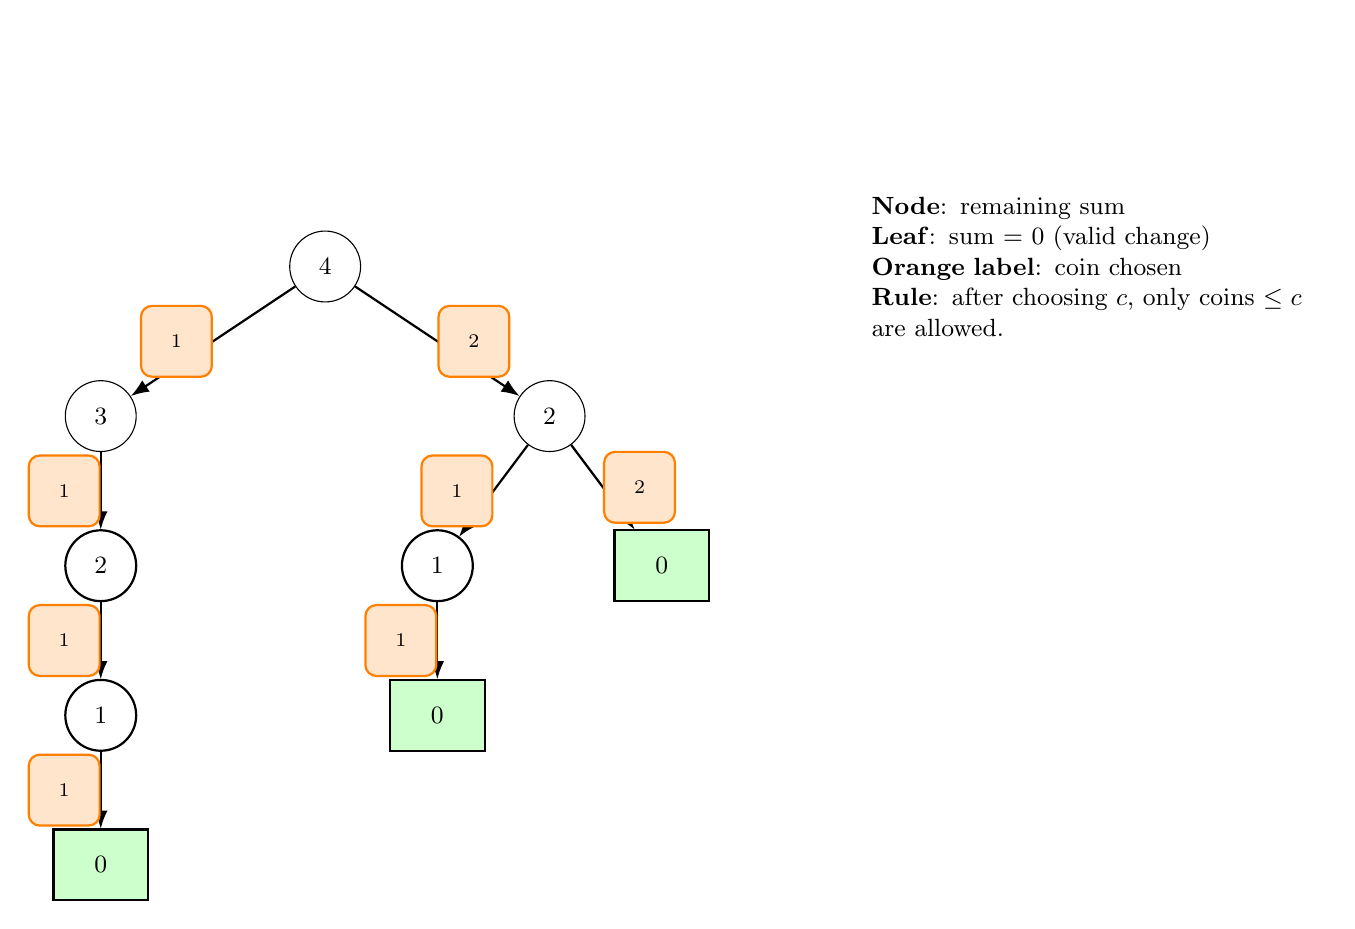
\begin{tikzpicture}[
    scale=0.95,
    level distance=2cm,
    level 1/.style={sibling distance=6cm},
    level 2/.style={sibling distance=3cm},
    level 3/.style={sibling distance=1.8cm},
    every node/.style={circle, draw, minimum size=0.9cm, font=\small},
    edge from parent/.style={draw, -{Latex}, thick},
    leaf/.style={rectangle, draw, fill=green!20, minimum width=1.2cm, font=\small},
    coin/.style={rectangle, rounded corners, draw=orange, fill=orange!20, font=\scriptsize, inner sep=2pt}
]

\node {4}
    child {
        node {3}
        child {
            node {2}
            child {
                node {1}
                child {
                    node[leaf] {0}
                    edge from parent node[coin, left] {1}
                }
                edge from parent node[coin, left] {1}
            }
            edge from parent node[coin, left] {1}
        }
        edge from parent node[coin, left] {1}
    }
    child {
        node {2}
        child {
            node {1}
            child {
                node[leaf] {0}
                edge from parent node[coin, left] {1}
            }
            edge from parent node[coin, left] {1}
        }
        child {
            node[leaf] {0}
            edge from parent node[coin, right] {2}
        }
        edge from parent node[coin, right] {2}
    };

% Legend — rapprochée du schéma
\node[draw=none, font=\small, anchor=west, align=left, text width=5.5cm] at (7, 0) {
    \textbf{Node}: remaining sum \\
    \textbf{Leaf}: sum = 0 (valid change) \\
    \textbf{Orange label}: coin chosen \\
    \textbf{Rule}: after choosing \(c\), only coins \(\leq c\) are allowed.
};

\end{tikzpicture}
\end{center}

The tree has 3 green leaves, corresponding to the 3 valid changes:
\begin{itemize}
    \item \( 1 + 1 + 1 + 1 \)
    \item \( 1 + 1 + 2 \)
    \item \( 2 + 2 \)
\end{itemize}

Note that \( 1 + 2 + 1 \) and \( 2 + 1 + 1 \) are \textbf{not} generated, because after choosing 2, the algorithm only allows coins \( \leq 2 \), and after choosing 1, it only allows coins \( \leq 1 \). The order is enforced to be non-increasing.

\subsubsection{Complexity}

Let \( S \) be the target sum, \( k \) the number of denominations, and \( c_{\min} \) the smallest coin. In any valid combination, a coin \( c_i \) can appear at most \( \lfloor S / c_i \rfloor \) times. Therefore, the total number of coins in a combination is at most:
\[
\sum_i \left\lfloor \frac{S}{c_i} \right\rfloor \leq k \cdot \left\lfloor \frac{S}{c_{\min}} \right\rfloor \leq k \cdot \frac{S}{c_{\min}}.
\]
The number of combinations is therefore bounded by:
\[
C(S, k) \leq k^{\lfloor S / c_{\min} \rfloor} \leq k^{S / c_{\min}}.
\]
If \( c_{\min} = 1 \) (which is the case for the European system), this simplifies to:
\[
C(S, k) \leq k^S.
\]
This is a \textbf{gross upper bound}: it counts all sequences of at most \( S \) coins, including invalid ones. But it is sufficient to show that the number of combinations is \textbf{exponential in \( S \)}.

\textbf{Time complexity.} The tree has at most \( \lfloor S / c_{\min} \rfloor + 1 \) levels, and each node has at most \( k \) children. The total number of nodes is at most:
\[
1 + k + k^2 + \dots + k^{\lfloor S / c_{\min} \rfloor} = O\left(k^{S / c_{\min}}\right).
\]
Therefore, the time complexity is:
\[
T(S, k) = O\left(k^{S / c_{\min}}\right).
\]
For the European system (\( c_{\min} = 1 \)), this is \( O(k^S) \).

\textbf{Space complexity.} The recursion stack has at most \( \lfloor S / c_{\min} \rfloor + 1 \) levels, so \( O(S / c_{\min}) \) space. The results are at most \( C(S, k) \leq k^{S / c_{\min}} \) combinations, each of size at most \( S / c_{\min} \), so \( O(S \cdot k^{S / c_{\min}}) \) space.


\subsection{When Is Greedy Optimal?}

A greedy algorithm is optimal if the problem has two properties:
\begin{enumerate}
    \item \textbf{Greedy choice property:} a locally optimal choice is part of some globally optimal solution.
    \item \textbf{Optimal substructure:} after making the greedy choice, the remaining problem is a smaller instance of the same problem.
\end{enumerate}

For the interested reader: the greedy algorithm is guaranteed to be optimal on any problem whose feasible sets form a \textbf{matroid} --- a combinatorial structure that generalizes linear independence (Edmonds, 1971). The coin change problem does not have this structure in general, which is why greedy can fail on non-canonical systems.

For the European coin system, both properties hold. For \(\{1, 3, 4\}\), the greedy choice property fails: taking 4 first is locally optimal (it reduces the sum the most), but it does not lead to a globally optimal solution.

\subsection{Summary}

\begin{center}
\begin{tabular}{lcc}
\toprule
Problem & Algorithm & Complexity \\
\midrule
Coin change (European) & Greedy & \(O(k)\) time, \(O(1)\) space \\
All possible changes & Backtracking & \(O(k^S)\) time, \(O(S)\) space \\
\bottomrule
\end{tabular}
\end{center}

\textbf{The lesson:} greedy is fast and simple, but it is not always correct. It must be \emph{proven} optimal (exchange argument) or replaced by a more general technique (dynamic programming, backtracking).

% ============================================================
% 9. DYNAMIC PROGRAMMING
% ============================================================
\section{Dynamic Programming}

\textbf{Dynamic programming} (DP) is a technique for solving problems that have two properties:
\begin{enumerate}
    \item \textbf{Optimal substructure:} the optimal solution is built from optimal solutions of subproblems.
    \item \textbf{Overlapping subproblems:} the same subproblems are solved multiple times if we use naive recursion.
\end{enumerate}

DP avoids recomputation by \textbf{storing the results} of subproblems and \textbf{reusing} them. This transforms exponential algorithms into polynomial ones.

\subsection{Two Forms of DP}

\begin{center}
\begin{tabular}{lcc}
\toprule
Form & Direction & Structure \\
\midrule
Memoization & Top-down & Recursion + cache \\
Tabulation & Bottom-up & Iteration + table \\
\bottomrule
\end{tabular}
\end{center}

\subsection{Generalized Coin Change (Arbitrary Coin System)}

\subsubsection{Statement}

Given a sum \(S\) and an \textbf{arbitrary} set of coin denominations, find the minimum number of coins needed to make \(S\).

Unlike the European system, the greedy algorithm may fail. We need a general algorithm that works for \emph{any} coin system.

\subsubsection{The DP Recurrence}

Let \(\mathrm{dp}[s]\) be the minimum number of coins needed to make the sum \(s\). Then:
\[
\mathrm{dp}[0] = 0, \qquad \mathrm{dp}[s] = 1 + \min_{c \leq s} \mathrm{dp}[s - c].
\]

The idea: to make \(s\), we choose a coin \(c\), and we add 1 to the optimal solution for \(s - c\).

\subsubsection{The Algorithm}

\begin{lstlisting}
def coin_change_dp(S, coins):
    dp = [float('inf')] * (S + 1)
    dp[0] = 0
    for s in range(1, S + 1):
        for c in coins:
            if c <= s:
                dp[s] = min(dp[s], dp[s - c] + 1)
    return dp[S]
\end{lstlisting}

\begin{example}
\(S = 6\), coins \(\{1, 3, 4\}\). The table is filled as follows:
\begin{center}
\begin{tabular}{c|ccccccc}
\toprule
\(s\) & 0 & 1 & 2 & 3 & 4 & 5 & 6 \\
\midrule
\(\mathrm{dp}[s]\) & 0 & 1 & 2 & 1 & 1 & 2 & 2 \\
\bottomrule
\end{tabular}
\end{center}
The result is \(\mathrm{dp}[6] = 2\) (3 + 3).
\end{example}

\subsubsection{Complexity}

\textbf{Time:} \(O(S \cdot k)\), where \(k\) is the number of denominations. For each sum (S values), we try each coin (k values).

\textbf{Space:} \(O(S)\) for the DP table.

\subsection{Counting Balanced Parentheses}

\subsubsection{Statement}

Given an integer \(n\), we want to \textbf{count} the number of strings of \(n\) pairs of well-balanced parentheses. A string is well-balanced if every opening parenthesis has a matching closing parenthesis, and the parentheses are properly nested.

\begin{example}
\(n = 1\): \code{()}. (1 string)

\(n = 2\): \code{(())}, \code{()()}. (2 strings)

\(n = 3\): \code{((()))}, \code{(()())}, \code{(())()}, \code{()(())}, \code{()()()}. (5 strings)
\end{example}

The number of balanced strings of \(n\) pairs is the \(n\)-th \textbf{Catalan number}:
\[
C_n = \frac{1}{n+1} \binom{2n}{n}.
\]

\subsubsection{The DP Recurrence}

Let \(\mathrm{dp}[n]\) be the number of balanced strings of \(n\) pairs. The first character must be \code{(}, and it matches some \code{)} at position \(2k+1\). The string is then:
\[
\texttt{(} \; \text{inside} \; \texttt{)} \; \text{after}
\]
where \texttt{inside} is a balanced string of \(k\) pairs, and \texttt{after} is a balanced string of \(n-1-k\) pairs.

Therefore:
\[
\mathrm{dp}[0] = 1, \qquad \mathrm{dp}[n] = \sum_{k=0}^{n-1} \mathrm{dp}[k] \cdot \mathrm{dp}[n-1-k].
\]

\subsubsection{The Algorithm}

\begin{lstlisting}
def count_parentheses(n):
    dp = [0] * (n + 1)
    dp[0] = 1
    for i in range(1, n + 1):
        for k in range(i):
            dp[i] += dp[k] * dp[i - 1 - k]
    return dp[n]
\end{lstlisting}

\begin{example}
\(n = 4\): the table is filled as follows:
\begin{center}
\begin{tabular}{c|ccccc}
\toprule
\(i\) & 0 & 1 & 2 & 3 & 4 \\
\midrule
\(\mathrm{dp}[i]\) & 1 & 1 & 2 & 5 & 14 \\
\bottomrule
\end{tabular}
\end{center}
The result is \(\mathrm{dp}[4] = 14\) (the 4th Catalan number).
\end{example}

\subsubsection{Complexity}

\textbf{Time:} \(O(n^2)\). The outer loop runs \(n\) times, and the inner loop runs up to \(n\) times.

\textbf{Space:} \(O(n)\) for the DP table.

\subsubsection{Connection to the Catalan Numbers}

The DP table computes the Catalan numbers:
\[
C_0 = 1, \quad C_1 = 1, \quad C_2 = 2, \quad C_3 = 5, \quad C_4 = 14, \quad C_5 = 42, \dots
\]
These numbers appear in many combinatorial problems: binary trees, triangulations, Dyck paths, etc.

The \emph{generation} of these strings (via backtracking) is covered in Section~10.

\subsection{Comparison: Balanced Parentheses vs Paths Under the Diagonal}

The problem of counting balanced parentheses is closely related to another classical problem: counting lattice paths that stay under the diagonal. The two problems share the same structure, and both are counted by the Catalan numbers.

\subsubsection{The Path Problem}

Consider a grid from \( (0,0) \) to \( (n,n) \). We want to count the number of paths that:
\begin{itemize}
    \item start at \( (0,0) \) and end at \( (n,n) \),
    \item move only right (R) or up (U),
    \item never go above the diagonal \( y = x \).
\end{itemize}

\begin{example}
For \( n = 3 \), the valid paths are:
\begin{itemize}
    \item RRRUUU
    \item RRURUU
    \item RRUURU
    \item RURURU
    \item RURRUU
\end{itemize}
There are 5 paths, which is \( C_3 = 5 \).
\end{example}

\subsubsection{\texorpdfstring{The Five Paths for \( n = 3 \)}{The Five Paths for n = 3}}

\begin{center}
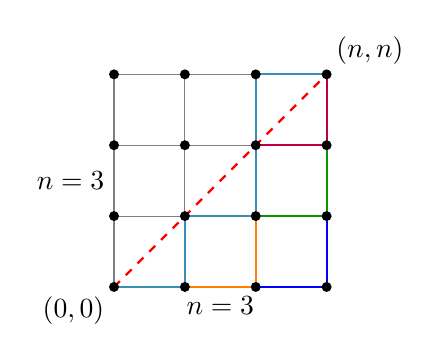
\begin{tikzpicture}[scale=0.9]
    % Grille
    \draw[gray, thin] (0,0) grid (3,3);
    
    % Diagonale
    \draw[thick, dashed, red] (0,0) -- (3,3);
    
    % Chemin 1 : RRRUUU
    \draw[thick, blue] (0,0) -- (1,0) -- (2,0) -- (3,0) -- (3,1) -- (3,2) -- (3,3);
    
    % Chemin 2 : RRURUU
    \draw[thick, green!60!black] (0,0) -- (1,0) -- (2,0) -- (2,1) -- (3,1) -- (3,2) -- (3,3);
    
    % Chemin 3 : RRUURU
    \draw[thick, orange] (0,0) -- (1,0) -- (2,0) -- (2,1) -- (2,2) -- (3,2) -- (3,3);
    
    % Chemin 4 : RURURU
    \draw[thick, purple] (0,0) -- (1,0) -- (1,1) -- (2,1) -- (2,2) -- (3,2) -- (3,3);
    
    % Chemin 5 : RURRUU
    \draw[thick, cyan!70!black] (0,0) -- (1,0) -- (1,1) -- (2,1) -- (2,2) -- (2,3) -- (3,3);
    
    % Points
    \foreach \x in {0,1,2,3} {
        \foreach \y in {0,1,2,3} {
            \fill[black] (\x,\y) circle (2pt);
        }
    }
    
    % Labels
    \node[below] at (1.5,0) {\(n = 3\)};
    \node[left] at (0,1.5) {\(n = 3\)};
    \node[below left] at (0,0) {\((0,0)\)};
    \node[above right] at (3,3) {\((n,n)\)};
\end{tikzpicture}
\end{center}

\subsubsection{The Correspondence}

There is a direct correspondence between balanced parentheses and paths under the diagonal:
\begin{itemize}
    \item An opening parenthesis \code{(} corresponds to a \textbf{right step} R.
    \item A closing parenthesis \code{)} corresponds to an \textbf{up step} U.
\end{itemize}

A path stays under the diagonal \( y = x \) if and only if, at every prefix, the number of up steps is at most the number of right steps. This is exactly the condition that a parenthesis string is balanced: at every prefix, the number of closing parentheses is at most the number of opening parentheses.

\begin{example}
The string \code{(()())} corresponds to the path R R U R U U, which stays under the diagonal.
\end{example}

The following table lists the five solutions for \( n = 3 \), side by side:

\begin{center}
\begin{tabular}{cc}
\toprule
Balanced parentheses & Path \\
\midrule
\code{((()))} & RRRUUU \\
\code{(()())} & RRURUU \\
\code{(())()} & RRUURU \\
\code{()(())} & RURURU \\
\code{()()()} & RURRUU \\
\bottomrule
\end{tabular}
\end{center}

\subsubsection{Why This Matters}

The two problems share the same structure: the same counters, the same rules, and the same number of solutions (the Catalan numbers). This means that an algorithm for one problem can be adapted to the other by a simple translation:
\begin{itemize}
    \item To \textbf{count} balanced parentheses, use the Catalan formula or the DP recurrence.
    \item To \textbf{count} paths under the diagonal, use the same formula or recurrence.
\end{itemize}

The \emph{generation} of both (via backtracking) is covered in Section~10.

\subsubsection{The Catalan Numbers}

Both problems are counted by the \( n \)-th Catalan number:
\[
C_n = \frac{1}{n+1} \binom{2n}{n}.
\]
The first values are:
\[
C_0 = 1, \quad C_1 = 1, \quad C_2 = 2, \quad C_3 = 5, \quad C_4 = 14, \quad C_5 = 42, \dots
\]
These numbers appear in many other problems: binary trees, triangulations of polygons, Dyck paths, and many more.

% ============================================================
% 10. BACKTRACKING
% ============================================================
\section{Backtracking}

\subsection{What Is Backtracking?}

\textbf{Backtracking} is a technique for exploring all possible solutions to a problem. It builds a solution \emph{incrementally}, and \textbf{abandons} a partial solution as soon as it determines that it cannot lead to a valid solution.

The general pattern is:
\begin{enumerate}
    \item \textbf{Choose} an option.
    \item \textbf{Explore} the consequences (recursively).
    \item \textbf{Undo} the choice (backtrack) and try another option.
\end{enumerate}

The key difference from simple recursion is the \textbf{undo} step: after exploring a branch, we restore the state to what it was before the choice, so that we can explore other branches.

\begin{example}[Maze]
In a maze, you try a direction. If you hit a dead end, you \emph{go back} to the previous intersection and try another direction. This is backtracking.
\end{example}

\subsection{Generating All Permutations}

\subsubsection{Statement}

Given an array of $n$ distinct elements, generate \textbf{all possible permutations}.

\begin{example}
For $[1, 2, 3]$, the permutations are:
\[
[1,2,3], \quad [1,3,2], \quad [2,1,3], \quad [2,3,1], \quad [3,1,2], \quad [3,2,1].
\]
There are $3! = 6$ permutations.
\end{example}

\subsubsection{The Algorithm}

We build the permutation incrementally: at each step, we choose an element from the remaining ones, and recurse. When no elements remain, we have a complete permutation.

\begin{lstlisting}
def permutations(arr):
    result = []

    def backtrack(current, remaining):
        if not remaining:
            result.append(current[:])
            return
        for i in range(len(remaining)):
            current.append(remaining[i])
            backtrack(current, remaining[:i] + remaining[i+1:])
            current.pop()   # undo (backtrack)

    backtrack([], arr)
    return result
\end{lstlisting}

\textbf{How it works.} The function \code{backtrack} takes the current permutation (\code{current}) and the elements not yet placed (\code{remaining}). If \code{remaining} is empty, the permutation is complete: we add a copy to the result. Otherwise, for each element in \code{remaining}, we place it at the end of \code{current}, recurse, and then \textbf{undo} the choice (\code{current.pop()}).

\subsubsection{Example: Tree for $[1, 2, 3]$}

\begin{center}
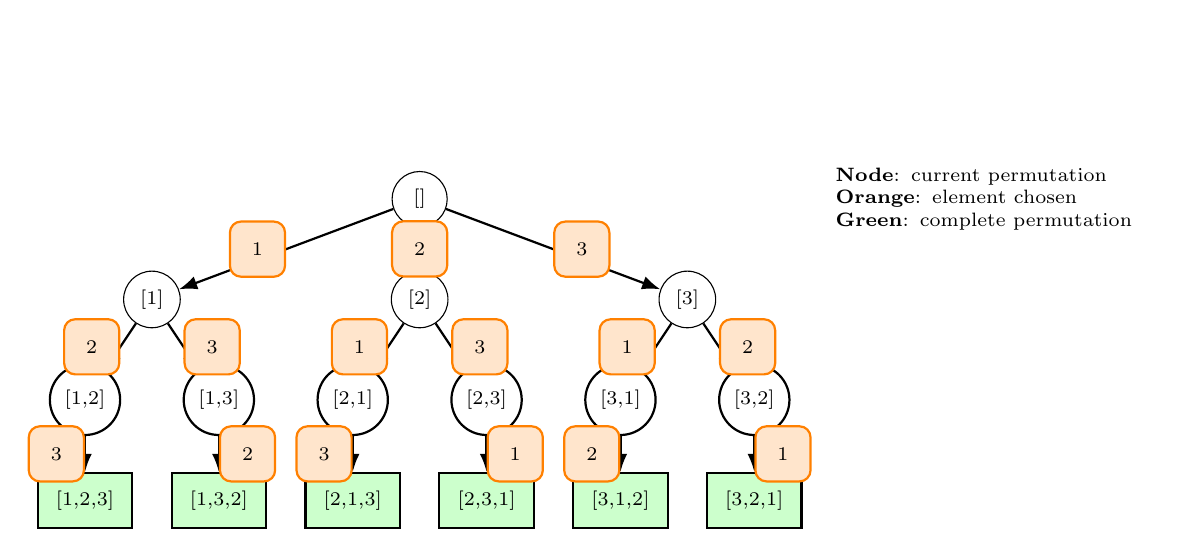
\begin{tikzpicture}[
    scale=0.85,
    level distance=1.5cm,
    level 1/.style={sibling distance=4cm},
    level 2/.style={sibling distance=2cm},
    level 3/.style={sibling distance=1.2cm},
    every node/.style={circle, draw, minimum size=0.7cm, font=\scriptsize},
    edge from parent/.style={draw, -{Latex}, thick},
    leaf/.style={rectangle, draw, fill=green!20, minimum width=1.2cm, font=\scriptsize},
    choice/.style={rectangle, rounded corners, draw=orange, fill=orange!20, font=\scriptsize, inner sep=1pt}
]

\node {[]}
    child {
        node {[1]}
        child {
            node {[1,2]}
            child {
                node[leaf] {[1,2,3]}
                edge from parent node[choice, left] {3}
            }
            edge from parent node[choice, left] {2}
        }
        child {
            node {[1,3]}
            child {
                node[leaf] {[1,3,2]}
                edge from parent node[choice, right] {2}
            }
            edge from parent node[choice, right] {3}
        }
        edge from parent node[choice, left] {1}
    }
    child {
        node {[2]}
        child {
            node {[2,1]}
            child {
                node[leaf] {[2,1,3]}
                edge from parent node[choice, left] {3}
            }
            edge from parent node[choice, left] {1}
        }
        child {
            node {[2,3]}
            child {
                node[leaf] {[2,3,1]}
                edge from parent node[choice, right] {1}
            }
            edge from parent node[choice, right] {3}
        }
        edge from parent node[choice] {2}
    }
    child {
        node {[3]}
        child {
            node {[3,1]}
            child {
                node[leaf] {[3,1,2]}
                edge from parent node[choice, left] {2}
            }
            edge from parent node[choice, left] {1}
        }
        child {
            node {[3,2]}
            child {
                node[leaf] {[3,2,1]}
                edge from parent node[choice, right] {1}
            }
            edge from parent node[choice, right] {2}
        }
        edge from parent node[choice, right] {3}
    };

% Legend
\node[draw=none, font=\scriptsize, anchor=west, align=left, text width=4cm] at (6, 0) {
    \textbf{Node}: current permutation \\
    \textbf{Orange}: element chosen \\
    \textbf{Green}: complete permutation
};

\end{tikzpicture}
\end{center}

The tree has 6 green leaves, corresponding to the 6 permutations.

\subsubsection{Complexity}

\textbf{Time:} $O(n \cdot n!)$, where $n!$ is the number of permutations and $n$ is the cost of copying each permutation.

\textbf{Space:} $O(n)$ for the recursion stack, plus $O(n \cdot n!)$ for storing the results.

\subsection{Generating Balanced Parentheses}

\subsubsection{Statement}

Given an integer $n$, generate all strings of $n$ pairs of well-balanced parentheses.

\begin{example}
$n = 1$: \code{()}. (1 string)

$n = 2$: \code{(())}, \code{()()}. (2 strings)

$n = 3$: \code{((()))}, \code{(()())}, \code{(())()}, \code{()(())}, \code{()()()}. (5 strings)
\end{example}

\subsubsection{The Algorithm}

We build the string incrementally. At each step, we can:
\begin{enumerate}
    \item Add \code{(} if we have used fewer than $n$ opening parentheses.
    \item Add \code{)} if the number of closing parentheses is strictly less than the number of opening parentheses.
\end{enumerate}

These two rules guarantee that we never exceed $n$ opening parentheses, and we never close more than we have opened.

\begin{lstlisting}
def generate(n):
    result = []

    def backtrack(current, open_count, close_count):
        if len(current) == 2 * n:
            result.append(current)
            return
        if open_count < n:
            backtrack(current + '(', open_count + 1, close_count)
        if close_count < open_count:
            backtrack(current + ')', open_count, close_count + 1)

    backtrack('', 0, 0)
    return result
\end{lstlisting}

\textbf{How it works.} The function \code{backtrack} takes the current string, the number of opening parentheses, and the number of closing parentheses. If the string has length $2n$, it is complete. Otherwise, we try to add \code{(} (if allowed) and \code{)} (if allowed), and recurse.

\subsubsection{Example: Tree for $n = 3$}

\begin{center}
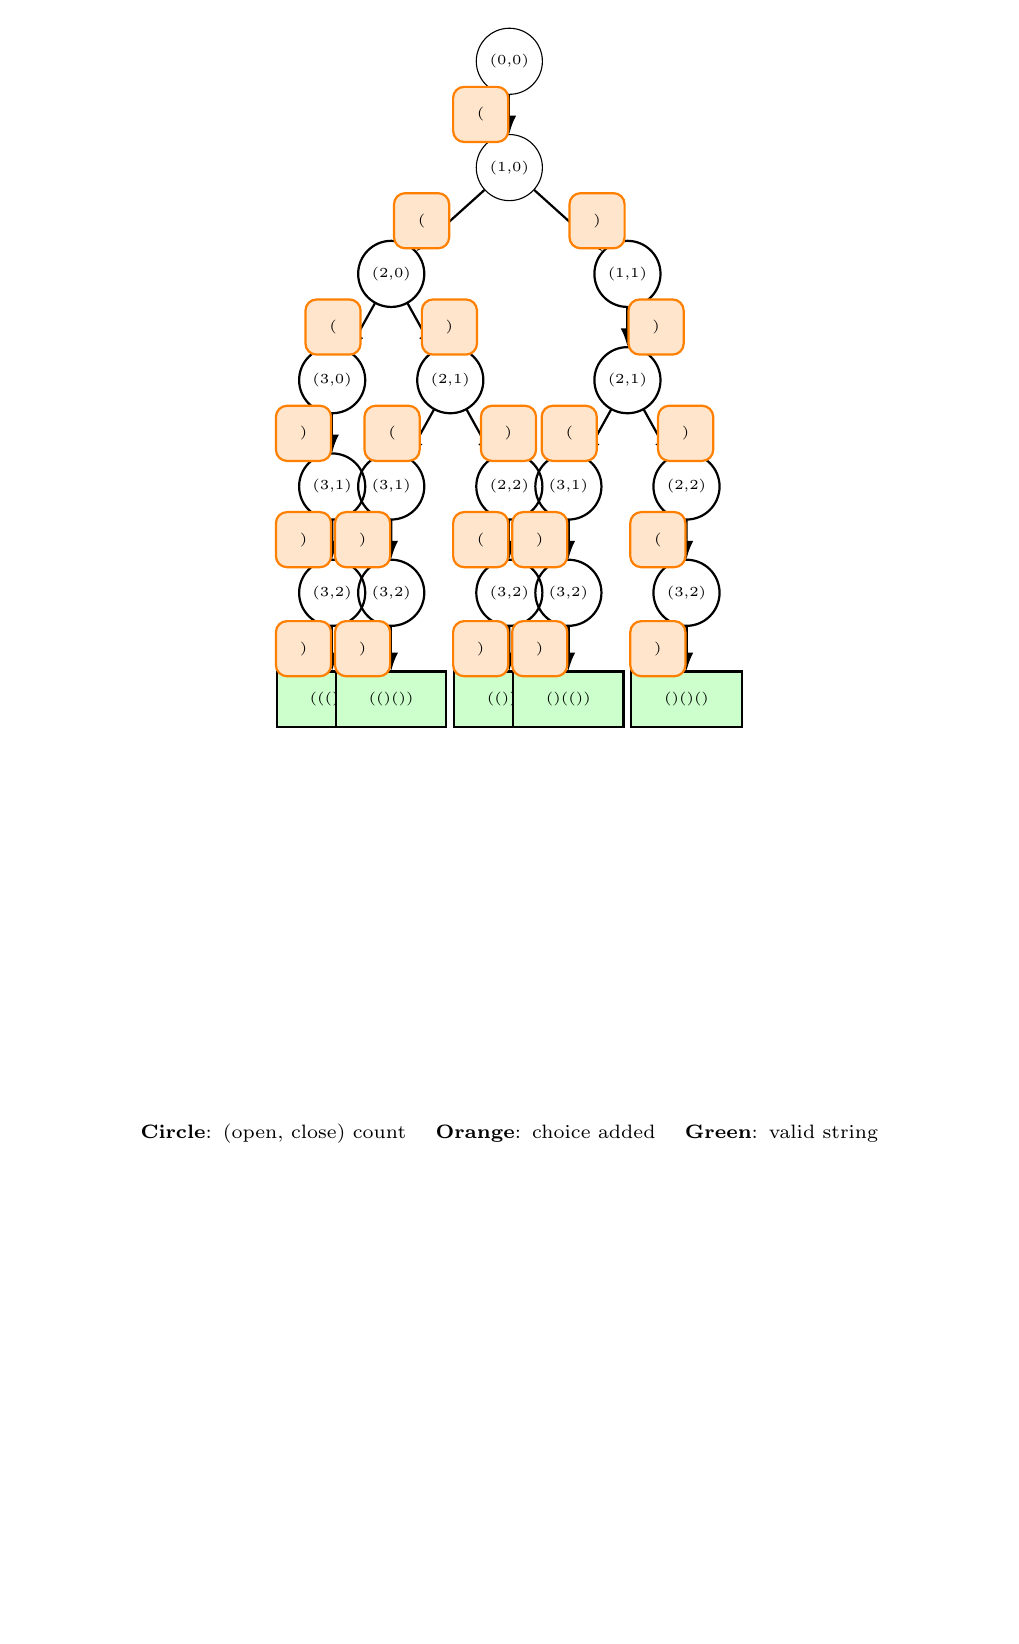
\begin{tikzpicture}[
    scale=0.75,
    level distance=1.8cm,
    level 1/.style={sibling distance=8cm},
    level 2/.style={sibling distance=4cm},
    level 3/.style={sibling distance=2cm},
    every node/.style={circle, draw, minimum size=0.7cm, font=\tiny},
    edge from parent/.style={draw, -{Latex}, thick},
    leaf/.style={rectangle, draw, fill=green!20, minimum width=1.4cm, font=\tiny},
    choice/.style={rectangle, rounded corners, draw=orange, fill=orange!20, font=\tiny, inner sep=1pt}
]

\node {(0,0)}
    child {
        node {(1,0)}
        child {
            node {(2,0)}
            child {
                node {(3,0)}
                child {
                    node {(3,1)}
                    child {
                        node {(3,2)}
                        child {
                            node[leaf] {((()))}
                            edge from parent node[choice, left] {)}
                        }
                        edge from parent node[choice, left] {)}
                    }
                    edge from parent node[choice, left] {)}
                }
                edge from parent node[choice, left] {(}
            }
            child {
                node {(2,1)}
                child {
                    node {(3,1)}
                    child {
                        node {(3,2)}
                        child {
                            node[leaf] {(()())}
                            edge from parent node[choice, left] {)}
                        }
                        edge from parent node[choice, left] {)}
                    }
                    edge from parent node[choice, left] {(}
                }
                child {
                    node {(2,2)}
                    child {
                        node {(3,2)}
                        child {
                            node[leaf] {(())()}
                            edge from parent node[choice, left] {)}
                        }
                        edge from parent node[choice, left] {(}
                    }
                    edge from parent node[choice, right] {)}
                }
                edge from parent node[choice, right] {)}
            }
            edge from parent node[choice, left] {(}
        }
        child {
            node {(1,1)}
            child {
                node {(2,1)}
                child {
                    node {(3,1)}
                    child {
                        node {(3,2)}
                        child {
                            node[leaf] {()(())}
                            edge from parent node[choice, left] {)}
                        }
                        edge from parent node[choice, left] {)}
                    }
                    edge from parent node[choice, left] {(}
                }
                child {
                    node {(2,2)}
                    child {
                        node {(3,2)}
                        child {
                            node[leaf] {()()()}
                            edge from parent node[choice, left] {)}
                        }
                        edge from parent node[choice, left] {(}
                    }
                    edge from parent node[choice, right] {)}
                }
                edge from parent node[choice, right] {)}
            }
            edge from parent node[choice, right] {)}
        }
        edge from parent node[choice, left] {(}
    };

% Legend
\node[draw=none, anchor=north, font=\scriptsize, text width=12cm, align=center] at (0, -10) {
    \textbf{Circle}: (open, close) count \quad
    \textbf{Orange}: choice added \quad
    \textbf{Green}: valid string
};

\end{tikzpicture}
\end{center}

The tree has 5 green leaves, corresponding to the 5 valid strings.

\subsubsection{Complexity}

\textbf{Time:} $O(C_n)$, where $C_n$ is the $n$-th Catalan number. Each valid string is generated exactly once.

\textbf{Space:} $O(n)$ for the recursion stack, plus $O(C_n \cdot n)$ for storing the results.

\subsection{The General Pattern}

All backtracking algorithms share the same structure:

\begin{lstlisting}
def backtrack(state):
    if is_solution(state):
        record(state)
        return
    for choice in choices(state):
        if is_valid(choice, state):
            make_choice(choice, state)
            backtrack(state)
            undo_choice(choice, state)
\end{lstlisting}

The three key steps are:
\begin{enumerate}
    \item \textbf{Choose}: try an option.
    \item \textbf{Explore}: recurse with the choice made.
    \item \textbf{Undo}: restore the state to try another option.
\end{enumerate}

The \textbf{undo} step is what distinguishes backtracking from simple recursion. Without it, the algorithm would not explore alternative branches.

\subsection{When to Use Backtracking}

Backtracking is the right choice when:
\begin{itemize}
    \item The problem asks to \textbf{enumerate} all solutions (permutations, combinations, paths).
    \item The problem has \textbf{constraints} that allow pruning (e.g., no two queens on the same diagonal).
    \item The search space is \textbf{exponential} but can be pruned effectively.
    \item There is no optimal substructure (so DP does not apply) and no greedy choice (so greedy does not apply).
\end{itemize}

Backtracking is \textbf{not} the right choice when:
\begin{itemize}
    \item The problem asks for the \textbf{minimum} or \textbf{maximum} (use DP or greedy instead).
    \item The search space is too large to explore (use heuristics or approximation).
    \item The problem has a polynomial-time algorithm (use it instead).
\end{itemize}

\subsection{Summary}

\begin{center}
\begin{tabular}{lcc}
\toprule
Problem & Paradigm & Complexity \\
\midrule
Generate permutations & Backtracking & $O(n \cdot n!)$ \\
Generate balanced parentheses & Backtracking & $O(C_n)$ \\
Count balanced parentheses & DP (Catalan) & $O(n)$ \\
\bottomrule
\end{tabular}
\end{center}

\textbf{The lesson:} backtracking is the tool for \emph{enumeration} problems. It explores all possibilities, but prunes branches that cannot lead to a solution. The key is the \textbf{undo} step.

% ============================================================
% 11. SUMMARY OF PARADIGMS
% ============================================================
\section{Summary of Algorithmic Paradigms}

The following table summarizes the four main algorithmic paradigms studied in this course.

\begin{center}
\renewcommand{\arraystretch}{1.3}
\small
\begin{tabular}{>{\raggedright\arraybackslash}p{2.5cm} >{\raggedright\arraybackslash}p{5cm} >{\raggedright\arraybackslash}p{4.5cm} >{\raggedright\arraybackslash}p{2.5cm}}
\toprule
Paradigm & Principle & Examples & Complexity \\
\midrule
\textbf{Divide and conquer} & Split into independent subproblems, solve recursively, combine & Merge sort, quick sort, dichotomy & $O(n \log n)$ \\
\textbf{Dynamic programming} & Split into overlapping subproblems, store results & Fibonacci, LCS, knapsack, coin change & Polynomial \\
\textbf{Greedy} & Make a locally optimal choice, never reconsider & Coin change, Interval Scheduling, Dijkstra & $O(n)$ to $O(n \log n)$ \\
\textbf{Backtracking} & Explore all possibilities, undo when stuck & Permutations, parentheses, N-Queens & Exponential \\
\bottomrule
\end{tabular}
\end{center}

\vspace{0.3cm}

The following table compares the paradigms on the key criteria.

\begin{center}
\renewcommand{\arraystretch}{1.3}
\small
\begin{tabular}{lcccc}
\toprule
Criterion & D\&C & DP & Greedy & Backtracking \\
\midrule
Subproblems & Independent & Overlapping & One remaining & Tree \\
Strategy & Split, solve, combine & Solve once, store & Choose, never return & Explore, undo \\
Memory & None & Table & None & Stack \\
Complexity & $O(n \log n)$ & Polynomial & $O(n) \text{ to } O(n \log n)$ & Exponential \\
Proof & Recurrence & Recurrence & Exchange argument & Correctness \\
\bottomrule
\end{tabular}
\end{center}

\textbf{The link between paradigms.} The four paradigms share the same idea --- \emph{decompose the problem} --- but differ in what they do with the subproblems:
\begin{itemize}
    \item \textbf{Divide and conquer}: solve them \emph{independently}.
    \item \textbf{Dynamic programming}: solve them \emph{once} and store the results.
    \item \textbf{Greedy}: choose \emph{one} and never return.
    \item \textbf{Backtracking}: explore \emph{all} of them and undo.
\end{itemize}

\newpage

% ============================================================
% APPENDIX A: RECURRENCES AND LOGARITHMS
% ============================================================

% Page de titre
\begin{center}
    \vspace*{5cm}
    {\Huge \textbf{Appendix}}\\[1cm]
    {\LARGE Recurrences and Logarithms}\\[2cm]
    {\large A Refresher for Students}
    \vfill
\end{center}

\newpage

\appendix
\section{Recurrences and Logarithms: A Refresher}

This appendix recalls the mathematical tools used throughout the course: arithmetic and geometric sequences, recurrences, and logarithms. Each section includes a proof of the main formula, so that the reader can see where the results come from.

\subsection{Arithmetic Sequences}

\begin{definition}[Arithmetic sequence]
A sequence $(u_n)$ is \textbf{arithmetic} if there is a constant $r$ (the \emph{common difference}) such that, for all $n$,
\[
u_{n+1} = u_n + r.
\]
The general term is:
\[
u_n = u_0 + n r.
\]
\end{definition}

\begin{example}
The sequence $1, 3, 5, 7, 9, \dots$ is arithmetic with $u_0 = 1$ and $r = 2$. Its general term is $u_n = 1 + 2n$.
\end{example}

\begin{theorem}[General term of an arithmetic sequence]
If a sequence $(u_n)$ satisfies $u_{n+1} = u_n + r$ for all $n$, with first term $u_0$, then:
\[
u_n = u_0 + n r.
\]
\end{theorem}

\begin{proof}
We prove the formula by induction on $n$.

\textbf{Base case.} For $n = 0$:
\[
u_0 + 0 \cdot r = u_0,
\]
which is the definition of the first term.

\textbf{Inductive step.} Assume that $u_k = u_0 + k r$ for some $k \geq 0$. We want to show that $u_{k+1} = u_0 + (k+1) r$. By the recurrence definition:
\[
u_{k+1} = u_k + r.
\]
Using the induction hypothesis $u_k = u_0 + k r$:
\[
u_{k+1} = (u_0 + k r) + r = u_0 + (k+1) r.
\]
This is exactly the formula for $n = k+1$.

By the principle of induction, the formula $u_n = u_0 + n r$ holds for all $n \geq 0$.
\end{proof}

\subsubsection{Sum of an Arithmetic Sequence}

\begin{theorem}[Sum of an arithmetic sequence]
For an arithmetic sequence $(u_n)$ with first term $u_0$ and common difference $r$, the sum of the first $n+1$ terms is:
\[
S_n = \sum_{k=0}^{n} u_k = (n+1) \cdot \frac{u_0 + u_n}{2}.
\]
\end{theorem}

\begin{proof}
We write the sum in two ways: in increasing order and in decreasing order.
\[
S_n = u_0 + u_1 + u_2 + \dots + u_n
\]
\[
S_n = u_n + u_{n-1} + u_{n-2} + \dots + u_0
\]
Adding the two lines term by term, we get:
\[
2 S_n = (u_0 + u_n) + (u_1 + u_{n-1}) + \dots + (u_n + u_0).
\]
Now, for every $k$, we have:
\[
u_k + u_{n-k} = (u_0 + k r) + (u_0 + (n-k) r) = 2 u_0 + n r = u_0 + u_n.
\]
So each of the $n+1$ terms in the sum equals $u_0 + u_n$. Therefore:
\[
2 S_n = (n+1)(u_0 + u_n),
\]
and dividing by 2 gives:
\[
S_n = (n+1) \cdot \frac{u_0 + u_n}{2}.
\]
\end{proof}

\begin{example}
The sum of the first $n+1$ integers is:
\[
0 + 1 + 2 + \dots + n = \frac{(n+1)n}{2}.
\]
This is the case $u_0 = 0$, $r = 1$, $u_n = n$.
\end{example}

\subsection{Geometric Sequences}

\begin{definition}[Geometric sequence]
A sequence $(u_n)$ is \textbf{geometric} if there is a constant $q$ (the \emph{common ratio}) such that, for all $n$,
\[
u_{n+1} = q \cdot u_n.
\]
The general term is:
\[
u_n = u_0 \cdot q^n.
\]
\end{definition}

\begin{example}
The sequence $1, 2, 4, 8, 16, \dots$ is geometric with $u_0 = 1$ and $q = 2$. Its general term is $u_n = 2^n$.
\end{example}

\begin{theorem}[General term of a geometric sequence]
If a sequence $(u_n)$ satisfies $u_{n+1} = q \cdot u_n$ for all $n$, with first term $u_0$, then:
\[
u_n = u_0 \cdot q^n.
\]
\end{theorem}

\begin{proof}
We prove the formula by induction on $n$.

\textbf{Base case.} For $n = 0$:
\[
u_0 \cdot q^0 = u_0 \cdot 1 = u_0,
\]
which is the definition of the first term.

\textbf{Inductive step.} Assume that $u_k = u_0 \cdot q^k$ for some $k \geq 0$. We want to show that $u_{k+1} = u_0 \cdot q^{k+1}$. By the recurrence definition:
\[
u_{k+1} = q \cdot u_k.
\]
Using the induction hypothesis $u_k = u_0 \cdot q^k$:
\[
u_{k+1} = q \cdot (u_0 \cdot q^k) = u_0 \cdot q^{k+1}.
\]
This is exactly the formula for $n = k+1$.

By the principle of induction, the formula $u_n = u_0 \cdot q^n$ holds for all $n \geq 0$.
\end{proof}

\subsubsection{Sum of a Geometric Sequence}

\begin{theorem}[Sum of a geometric sequence]
For a geometric sequence $(u_n)$ with first term $u_0$ and common ratio $q \neq 1$, the sum of the first $n+1$ terms is:
\[
S_n = \sum_{k=0}^{n} u_k = u_0 \cdot \frac{1 - q^{n+1}}{1 - q}.
\]
If $q = 1$, then $S_n = (n+1) u_0$.
\end{theorem}

\begin{proof}
We write the sum and multiply it by $q$:
\[
S_n = u_0 + u_0 q + u_0 q^2 + \dots + u_0 q^n
\]
\[
q S_n = u_0 q + u_0 q^2 + u_0 q^3 + \dots + u_0 q^{n+1}
\]
Subtracting the second line from the first, most terms cancel:
\[
S_n - q S_n = u_0 - u_0 q^{n+1}.
\]
Factoring:
\[
S_n (1 - q) = u_0 (1 - q^{n+1}).
\]
If $q \neq 1$, dividing by $1 - q$ gives:
\[
S_n = u_0 \cdot \frac{1 - q^{n+1}}{1 - q}.
\]
\end{proof}

\begin{example}[Binary tree]
A complete binary tree of height $h$ has $2^{h+1} - 1$ nodes. This is the geometric sum:
\[
1 + 2 + 4 + \dots + 2^h = \frac{2^{h+1} - 1}{2 - 1} = 2^{h+1} - 1.
\]
\end{example}

\begin{example}[Merge sort]
The recurrence $T(n) = 2T(n/2) + n$ has a recurrence tree where each level costs $n$. There are $\log_2 n$ levels, so the total is $n \log_2 n$.
\end{example}

\subsection{Solving Recurrences}

A \textbf{recurrence} is an equation that defines a sequence in terms of previous values. In algorithm analysis, recurrences express the running time of a recursive algorithm.

\begin{example}[Merge sort]
\[
T(n) = 2T(n/2) + O(n), \quad T(1) = O(1).
\]
\end{example}

\subsubsection{The Substitution Method}

We guess the solution and prove it by induction.

\begin{example}
Solve $T(n) = 2T(n/2) + n$.

\textbf{Guess:} $T(n) = O(n \log n)$.

\textbf{Proof by induction.} Assume $T(k) \leq c k \log k$ for all $k < n$. Then:
\[
T(n) = 2T(n/2) + n \leq 2 \cdot c \frac{n}{2} \log \frac{n}{2} + n = c n (\log n - 1) + n = c n \log n - c n + n.
\]
For $c \geq 1$, $-cn + n \leq 0$, so $T(n) \leq c n \log n$.
\end{example}

\subsubsection{The Recurrence Tree Method}

We draw the recursion as a tree and sum the work at each level.

\begin{example}
Solve $T(n) = 2T(n/2) + n$.

\begin{center}
\begin{tikzpicture}[level distance=1cm, level 1/.style={sibling distance=4cm}, level 2/.style={sibling distance=2cm}]
\node {\(n\)}
    child {node {\(n/2\)}
        child {node {\(n/4\)}}
        child {node {\(n/4\)}}
    }
    child {node {\(n/2\)}
        child {node {\(n/4\)}}
        child {node {\(n/4\)}}
    };
\end{tikzpicture}
\end{center}

At each level, the total work is $n$ (the sum of the subproblems). There are $\log_2 n$ levels. Therefore:
\[
T(n) = n \cdot \log_2 n = O(n \log n).
\]
\end{example}

\subsection{Logarithms}

The \textbf{logarithm} of $x$ in base $b$, denoted $\log_b x$, is the exponent to which $b$ must be raised to obtain $x$:
\[
\log_b x = y \quad \Longleftrightarrow \quad b^y = x.
\]

\textbf{Key properties:}
\begin{itemize}
    \item $\log_b (xy) = \log_b x + \log_b y$ (product rule)
    \item $\log_b (x/y) = \log_b x - \log_b y$ (quotient rule)
    \item $\log_b (x^k) = k \log_b x$ (power rule)
    \item $\log_b x = \frac{\log_c x}{\log_c b}$ (change of base)
    \item $b^{\log_b x} = x$ (inverse)
\end{itemize}

\subsubsection{Why Logarithms Matter in Complexity}

Logarithms appear whenever an algorithm \textbf{halves} (or divides by a constant) the input at each step.

\begin{example}[Dichotomy]
At each step, the search space is halved. Starting with $n$ elements, after $k$ steps at most $n/2^k$ remain. To reach 1 element, we need $k \geq \log_2 n$. There'fore the complexity is $O(\log n)$.
\end{example}

\begin{example}[Merge sort]
The recursion tree has $\log_2 n$ levels. Each level costs $O(n)$. Therefore $O(n \log n)$.
\end{example}

\textbf{The base of the logarithm does not matter asymptotically}, because $\log_b n = \frac{\log_2 n}{\log_2 b}$, and $\frac{1}{\log_2 b}$ is a constant. So $O(\log_b n) = O(\log_2 n) = O(\log n)$ for any base $b > 1$.

\end{document}